\documentclass[12pt,a4paper]{article}

\usepackage{fontspec}
\XeTeXlinebreaklocale "th"
\XeTeXlinebreakskip = 0pt plus 1pt
\defaultfontfeatures{Ligatures=TeX}
\setmainfont[
  Path={fonts/TH Sarabun PSK V-1/},
  Extension=.ttf,
  UprightFont={*},
  BoldFont={* Bold},
  ItalicFont={* Italic},
  BoldItalicFont={* BoldItalic}
]{THSarabun}
\setmonofont{Latin Modern Mono}

\usepackage{graphicx}
\usepackage{amsmath}
\usepackage{amssymb}
\usepackage{geometry}
\usepackage{booktabs}
\usepackage{array}
\usepackage{tabularx}
\usepackage{hyperref}
\usepackage{fancyhdr}
\usepackage{listings}
\usepackage{xcolor}
\usepackage{float}
\usepackage{caption}
\usepackage{subcaption}
\usepackage{tikz}
\usetikzlibrary{arrows.meta,positioning,calc,decorations.pathreplacing}

\geometry{margin=1in}
\emergencystretch=2em
\setlength{\headheight}{14.5pt}
\linespread{1.15}
\pagestyle{fancy}
\fancyhf{}
\rhead{\thepage}
\lhead{เสถียรภาพสัญญาณเล็ก}

\hypersetup{
    unicode=true,
    colorlinks=true,
    linkcolor=blue,
    urlcolor=blue,
    citecolor=blue
}

\renewcommand{\abstractname}{บทคัดย่อ}
\renewcommand{\contentsname}{สารบัญ}
\renewcommand{\figurename}{รูปที่}
\renewcommand{\tablename}{ตารางที่}
\renewcommand{\refname}{เอกสารอ้างอิง}

\lstset{
    basicstyle=\ttfamily\small,
    keywordstyle=\color{blue},
    stringstyle=\color{red},
    commentstyle=\color{green!60!black},
    frame=single,
    breaklines=true,
    postbreak=\mbox{\textcolor{red}{$\hookrightarrow$}\space},
    showstringspaces=false
}

\newcommand{\dwr}{\Delta\omega_r}
\newcommand{\ddel}{\Delta\delta}
\newcommand{\dpsifd}{\Delta\psi_{fd}}

\title{\textbf{การวิเคราะห์เสถียรภาพสัญญาณเล็กและการจำลอง MATLAB\\
ของระบบเครื่องกำเนิดเดี่ยวต่อบัสอนันต์}\\
\large อ้างอิง Kundur, \textit{Power System Stability and Control}, บทที่ 12}
\author{การศึกษาเสถียรภาพระบบไฟฟ้ากำลัง --- บทที่ 12}
\date{31 พฤษภาคม 2569}

\raggedbottom

\begin{document}

\maketitle
\thispagestyle{empty}

\begin{abstract}
ระบบเครื่องกำเนิดเดี่ยวต่อบัสอนันต์ (single-machine infinite-bus: SMIB)
คือแบบจำลองมาตรฐานสำหรับศึกษาความเสถียรของมุมโรเตอร์ภายใต้สัญญาณรบกวนขนาดเล็ก
โดยแทนเครื่องกำเนิดซิงโครนัสที่ต่อผ่านรีแอกแตนซ์สมมูลไปยังบัสอุดมคติซึ่งมีแรงดันและความถี่คงที่
\emph{เสถียรภาพสัญญาณเล็ก} หมายถึงความสามารถของเครื่องในการคงสภาพซิงโครไนซ์หลังเกิดการรบกวนขนาดเล็ก
เนื่องจากการรบกวนมีขนาดเล็ก สมการระบบจึงสามารถลิเนียไรซ์รอบจุดทำงาน และตัดสินเสถียรภาพจากค่าลักษณะเฉพาะของเมทริกซ์สถานะที่ได้
รายงานนี้วิเคราะห์ระบบ SMIB ตาม Kundur, \textit{Power System Stability and Control}, บทที่ 12 ที่ระดับรายละเอียด 4 ระดับ ได้แก่
แบบจำลอง \emph{classical} (ฟลักซ์คงที่หลังรีแอกแตนซ์ชั่วครู่),
แบบจำลอง \emph{field-circuit} (เพิ่มพลวัตฟลักซ์สนาม),
แบบจำลอง \emph{AVR} (เพิ่มตัวกระตุ้นไทริสเตอร์และตัวควบคุมแรงดันอัตโนมัติ),
และแบบจำลอง \emph{AVR\,+\,PSS} (เพิ่ม power system stabilizer)
สำหรับแต่ละแบบจำลอง รายงานสร้างแบบจำลอง state-space ที่ลิเนียไรซ์แล้ว คำนวณค่าลักษณะเฉพาะ
และประเมินอัตราส่วนการหน่วงกับความถี่การสั่น พร้อมใช้ผลตอบสนองในโดเมนเวลาเพื่อยืนยันคำทำนายจากค่าลักษณะเฉพาะ
ผลหลักที่ได้สอดคล้องกับตัวอย่างใน Kundur บทที่ 12: ความถี่สวิงเชิงกลไฟฟ้าแบบ classical เท่ากับ $1.02$~Hz,
พลวัตวงจรสนามให้การหน่วงบวกเล็กน้อย,
AVR อัตราขยายสูงเมื่อ $K_5$ เป็นลบจะ \emph{ลด} แรงบิดหน่วงและทำให้โหมดสวิงไม่เสถียร
(ค่าลักษณะเฉพาะ $+0.504\pm j7.23$),
และ PSS ที่ปรับแต่งเหมาะสมจะคืนการหน่วงบวกและย้ายโหมดสวิงกลับสู่ครึ่งระนาบซ้าย
($-1.005\pm j6.607$, $\zeta=0.15$)
\end{abstract}
\newpage
\tableofcontents
\newpage

\section{บทนำ}

เสถียรภาพสัญญาณเล็กคือความสามารถของระบบไฟฟ้ากำลังในการรักษาสภาวะซิงโครไนซ์เมื่อถูกรบกวนเล็กน้อย
เช่น การเปลี่ยนแปลงโหลดหรือกำลังผลิตแบบเพิ่มขึ้นเล็กน้อย
เมื่อการรบกวนมีขนาดเล็ก สมการไม่เชิงเส้นของระบบสามารถลิเนียไรซ์รอบจุดทำงานสภาวะคงตัวได้
จากนั้นเสถียรภาพจะถูกกำหนดโดยค่าลักษณะเฉพาะของเมทริกซ์สถานะที่ลิเนียไรซ์แล้ว:
ระบบมีเสถียรภาพสัญญาณเล็กก็ต่อเมื่อค่าลักษณะเฉพาะทุกค่ามีส่วนจริงเป็นลบ

ประเด็นเด่นสำหรับเครื่องกำเนิดซิงโครนัสที่ต่อกับกริดขนาดใหญ่คือโหมด
\textit{เชิงกลไฟฟ้า} หรือ \textit{สวิง} ซึ่งเป็นการสั่นของโรเตอร์เทียบกับส่วนที่เหลือของระบบ
โดยมักอยู่ในช่วง $0.1$--$2$~Hz
ลักษณะของโหมดนี้ถูกกำหนดโดยองค์ประกอบแรงบิดสองส่วนที่กระทำต่อโรเตอร์:
\textit{แรงบิดซิงโครไนซ์} ซึ่งอยู่เฟสเดียวกับการเบี่ยงเบนมุมโรเตอร์ $\ddel$
และ \textit{แรงบิดหน่วง} ซึ่งอยู่เฟสเดียวกับการเบี่ยงเบนความเร็ว $\dwr$
แรงบิดซิงโครไนซ์ไม่เพียงพอทำให้เกิดความไม่เสถียรแบบไม่สั่น (monotonic instability)
ส่วนแรงบิดหน่วงไม่เพียงพอทำให้เกิดการสั่นที่ขยายตัว

รายงานนี้ศึกษารูปแบบมาตรฐานทั้งสี่ของระบบ SMIB ใน Kundur บทที่ 12
สำหรับแต่ละกรณีจะประกอบเมทริกซ์สถานะลิเนียไรซ์ คำนวณโครงสร้างค่าลักษณะเฉพาะ
ตีความผลในเชิงกายภาพ และตรวจสอบกับค่าจากตำรา
การวิเคราะห์ถูกนำไปทำซ้ำเชิงตัวเลขใน MATLAB โดยสรุปการใช้งานไว้ในหัวข้อ~\ref{sec:impl}
แต่จุดเน้นของรายงานอยู่ที่การวิเคราะห์เสถียรภาพเอง

\section{วัตถุประสงค์}

\begin{enumerate}
    \item นำเสนอระบบ SMIB และความหมายของเสถียรภาพสัญญาณเล็กสำหรับพลวัตมุมโรเตอร์
    \item พัฒนาแบบจำลอง state-space ที่ลิเนียไรซ์ของเครื่องกำเนิดใน 4 ระดับรายละเอียด:
          classical, field-circuit, AVR และ AVR\,+\,PSS
    \item อนุมานค่าคงที่ Heffron--Phillips $K$ จากพารามิเตอร์พื้นฐานของเครื่องบนแกน
          $d$--$q$ รวมถึงผลอิ่มตัวแม่เหล็ก
    \item ประเมินเสถียรภาพด้วยค่าลักษณะเฉพาะ อัตราส่วนการหน่วง และความถี่ธรรมชาติ
          พร้อมยืนยันข้อสรุปด้วยผลตอบสนองในโดเมนเวลา
    \item แสดงผลของ AVR และบทบาทแก้ไขของ PSS ต่อโหมดสวิง
          และตรวจสอบผลทุกกรณีกับ Kundur บทที่ 12
\end{enumerate}

\section{ระบบเครื่องกำเนิดเดี่ยวต่อบัสอนันต์}
\label{sec:smib}

ระบบเครื่องกำเนิดเดี่ยวต่อบัสอนันต์ (SMIB) แทนเครื่องกำเนิดซิงโครนัสหนึ่งเครื่อง
ที่ต่อผ่านหม้อแปลงและสายส่งซึ่งรวมเป็นรีแอกแตนซ์สมมูล ไปยังระบบไฟฟ้าขนาดใหญ่มาก
ระบบขนาดใหญ่นี้ถูกอุดมคติให้เป็น \emph{บัสอนันต์}: แหล่งจ่ายที่มีขนาดแรงดันคงที่
ความถี่คงที่ และมุมเฟสคงที่ โดยไม่ได้รับผลกระทบจากพฤติกรรมของเครื่องกำเนิดเดี่ยว
ดังนั้นบัสอนันต์จึงเป็นแกนอ้างอิงของมุมและความถี่ที่โรเตอร์ของเครื่องกำเนิดสวิงเทียบอยู่

ในรูปแทนแบบ classical เครื่องกำเนิดถูกแทนด้วยแรงดันภายในคงที่
$E'\angle\delta$ หลังรีแอกแตนซ์ชั่วครู่ $X_d'$ และเครือข่ายภายนอกเป็นรีแอกแตนซ์อนุกรม $X_E$
มุมโรเตอร์ $\delta$ คือมุมของแรงดันภายในเทียบกับแรงดันบัสอนันต์ $E_B\angle 0^\circ$
ดังแสดงในรูปที่~\ref{fig:smib}

\begin{figure}[H]
\centering
\begin{tikzpicture}[font=\small,>=Latex]
\draw[thick] (0,0) circle (0.6);
\node at (0,0) {$E'\angle\delta$};
\node[below=2pt] at (0,-0.6) {แรงดันภายใน};
\draw[thick] (0.6,0) -- (1.6,0);
\draw[thick] (1.6,-0.25) rectangle (2.6,0.25);
\node at (2.1,0) {$jX_d'$};
\draw[thick] (2.6,0) -- (3.4,0);
\draw[thick] (3.4,-0.25) rectangle (4.4,0.25);
\node at (3.9,0) {$jX_E$};
\draw[thick] (4.4,0) -- (5.6,0);
\draw[line width=2pt] (5.6,-0.7) -- (5.6,0.7);
\node[right=2pt,align=left] at (5.6,0) {$E_B\angle 0^\circ$\\[-1pt]\scriptsize บัสอนันต์};
\draw[->] (3.0,0.35) -- (3.6,0.35);
\node at (3.3,0.6) {$I_t$};
\draw[decorate,decoration={brace,amplitude=5pt,mirror}] (1.6,-0.55) -- (4.4,-0.55);
\node[below=6pt] at (3.0,-0.55) {$X_T = X_d' + X_E$};
\end{tikzpicture}
\caption{ระบบเครื่องกำเนิดเดี่ยวต่อบัสอนันต์ เครื่องกำเนิดถูกแทนด้วยแรงดันคงที่
$E'$ หลังรีแอกแตนซ์ชั่วครู่ $X_d'$ ต่อผ่านรีแอกแตนซ์ภายนอก $X_E$
ไปยังบัสอนันต์ที่มีแรงดันคงที่ $E_B\angle 0^\circ$
มุมโรเตอร์ $\delta$ วัดเทียบกับแกนอ้างอิงของบัสอนันต์ และรีแอกแตนซ์รวมคือ
$X_T = X_d' + X_E$}
\label{fig:smib}
\end{figure}

ระบบ SMIB ถูกใช้เป็นแบบจำลองมาตรฐานของเสถียรภาพมุมโรเตอร์สัญญาณเล็ก
เพราะแยกปฏิสัมพันธ์เชิงกลไฟฟ้าระหว่างเครื่องกำเนิดหนึ่งเครื่องกับกริดออกมาได้
ขณะเดียวกันยังมีอันดับต่ำพอให้วิเคราะห์เชิงปิดได้
แบบจำลองนี้เป็นจุดเริ่มต้นของแบบจำลองเครื่องจักรลิเนียไรซ์ในเอกสารมาตรฐานด้านพลวัตระบบไฟฟ้า~\cite{kundur,anderson,sauer}
กลไกทางกายภาพที่แบบจำลองเผยให้เห็น เช่น แรงบิดซิงโครไนซ์และแรงบิดหน่วง
ผลทำลายเสถียรภาพของการควบคุมแรงดันอัตราขยายสูง และบทบาทแก้ไขของ power system stabilizer
สามารถถ่ายโอนไปยังเครื่องกำเนิดในระบบหลายเครื่องได้โดยตรง

\section{การสร้างแบบจำลองทางคณิตศาสตร์}
\label{sec:model}

\subsection{ความสัมพันธ์กำลัง-มุม}

เมื่อแทนเครื่องกำเนิดเป็น $E'\angle\delta$ หลัง $X_d'$ และแทนเครือข่ายเป็น $X_E$
กำลังช่องว่างอากาศหรือกำลังไฟฟ้าที่ส่งไปยังบัสอนันต์คือ

\begin{equation}
P_e = \frac{E' E_B}{X_T}\sin\delta,
\qquad X_T = X_d' + X_E.
\label{eq:Pe}
\end{equation}

สมการนี้คือกราฟกำลัง-มุม: กำลังส่งเพิ่มตามมุมโรเตอร์จนถึง $\delta = 90^\circ$
ความชันของกราฟที่จุดทำงานกำหนดว่าเครื่องต้านการเปลี่ยนมุมได้แรงเพียงใด
ซึ่งก็คือแรงบิดซิงโครไนซ์

\subsection{สมการสวิง}

การเคลื่อนที่ของโรเตอร์ถูกกำหนดโดยสมการสวิง ซึ่งสมดุลแรงบิดเร่ง
(อินพุตเชิงกลลบเอาต์พุตไฟฟ้า) กับความเฉื่อยของโรเตอร์:

\begin{equation}
\frac{2H}{\omega_0}\frac{d^2\delta}{dt^2}
= T_m - T_e - K_D\,\Delta\omega_r,
\label{eq:swing}
\end{equation}

โดย $H$ คือค่าคงที่ความเฉื่อย, $\omega_0 = 2\pi f_0$ คือความเร็วไฟฟ้าฐาน,
$K_D$ คือสัมประสิทธิ์การหน่วง และ $\Delta\omega_r$ คือการเบี่ยงเบนความเร็วแบบ per-unit
ใกล้ความเร็วซิงโครนัส แรงบิดเชิงกลและไฟฟ้าเกือบเท่ากับกำลังที่สอดคล้องกันในระบบ per unit

\subsection{การลิเนียไรซ์}

สำหรับการเบี่ยงเบนขนาดเล็กรอบจุดทำงาน $\delta_0$ กำลังไฟฟ้าในสมการ~\eqref{eq:Pe}
ถูกลิเนียไรซ์เป็น

\begin{equation}
\Delta P_e
= \left.\frac{\partial P_e}{\partial \delta}\right|_{\delta_0}\!\ddel
= \underbrace{\frac{E' E_B}{X_T}\cos\delta_0}_{K_S}\,\ddel
= K_S\,\ddel,
\label{eq:Ks}
\end{equation}

โดย $K_S$ คือ \textit{สัมประสิทธิ์แรงบิดซิงโครไนซ์}
เมื่อนำกำลังที่ลิเนียไรซ์แล้วแทนในสมการสวิง และเขียนการเบี่ยงเบนมุมกับความเร็วโรเตอร์เป็นสถานะ
จะได้แบบจำลอง state-space ต่อไปนี้

\subsection{แบบจำลอง State-Space: Classical}

เมื่อแทนเครื่องกำเนิดด้วยแรงดันคงที่ $E'$ หลัง $X_d'$ สมการสวิงลิเนียไรซ์คือ
(Kundur สมการ~12.78):

\begin{equation}
\frac{d}{dt}
\begin{bmatrix} \dwr \\ \ddel \end{bmatrix}
=
\begin{bmatrix}
-\dfrac{K_D}{2H} & -\dfrac{K_S}{2H} \\[2ex]
\omega_0 & 0
\end{bmatrix}
\begin{bmatrix} \dwr \\ \ddel \end{bmatrix}
+
\begin{bmatrix} \dfrac{1}{2H} \\[2ex] 0 \end{bmatrix}
\Delta T_m.
\label{eq:classA}
\end{equation}

ความถี่ธรรมชาติแบบไม่หน่วงและอัตราส่วนการหน่วงได้จากสมการลักษณะเฉพาะของสมการ~\eqref{eq:classA}:

\begin{equation}
\omega_n = \sqrt{\frac{K_S\,\omega_0}{2H}},
\qquad
\zeta = \frac{1}{2}\,\frac{K_D}{2H\,\omega_n}.
\label{eq:wn}
\end{equation}

\subsection{แบบจำลอง State-Space: พลวัตวงจรสนาม}

การเพิ่มฟลักซ์ลิงก์ของขดลวดสนาม $\dpsifd$ เป็นสถานะที่สาม
ทำให้แบบจำลองจับผลลดแม่เหล็กอย่างช้าๆ จากปฏิกิริยาอาร์เมเจอร์ได้
เมทริกซ์สถานะจึงเป็น (Kundur สมการ~12.116):

\begin{equation}
A_B =
\begin{bmatrix}
-\dfrac{K_D}{2H} & -\dfrac{K_1}{2H} & -\dfrac{K_2}{2H} \\[2ex]
\omega_0 & 0 & 0 \\[1ex]
0 & a_{32} & a_{33}
\end{bmatrix},
\end{equation}

โดย $K_1$ คือสัมประสิทธิ์แรงบิดซิงโครไนซ์เมื่อฟลักซ์คงที่,
$K_2$ เชื่อมโยงแรงบิดไฟฟ้ากับฟลักซ์สนาม และสมาชิกของสมการสนามคือ
$a_{32} = -K_3 K_4 / T_3$, $a_{33} = -1/T_3$
ค่าคงที่ $K_1$--$K_4$ และค่าคงที่เวลาเชิงผล $T_3$
ถูกอนุมานจากพารามิเตอร์ $d$--$q$ ในหัวข้อ~\ref{sec:kderiv}

\subsection{แบบจำลอง State-Space: ตัวกระตุ้นและ AVR}

ตัวกระตุ้นไทริสเตอร์ (Kundur type ST1A) ที่มีอัตราขยาย $K_A$
และตัวแปลงสัญญาณแรงดันปลายทางที่มีค่าคงที่เวลา $T_R$ เพิ่มสถานะที่สี่คือ $\Delta v_1$
ต้องใช้ค่าคงที่เพิ่มอีกสองค่า ได้แก่ $K_5$ (การเปลี่ยนแรงดันปลายทางเมื่อมุมโรเตอร์เปลี่ยน)
และ $K_6$ (การเปลี่ยนแรงดันปลายทางเมื่อฟลักซ์สนามเปลี่ยน)
แถวของสมการสนามและตัวแปลงสัญญาณคือ

\begin{equation}
a_{34} = -\frac{K_3}{T_3}K_A,
\qquad
\dot{\Delta v_1} = \frac{K_5}{T_R}\ddel + \frac{K_6}{T_R}\dpsifd
- \frac{1}{T_R}\Delta v_1.
\end{equation}

ผลตอบสนองฟลักซ์สนามต่อการรบกวนมุมโรเตอร์ เมื่อรวมการทำงานของตัวกระตุ้น คือ
(Kundur สมการ~12.144 โดย $G_{ex}(s)=K_A$):

\begin{equation}
\frac{\dpsifd}{\ddel}(s) =
\frac{-K_3\bigl[K_4(1+sT_R) + K_5 K_A\bigr]}
     {(1+sT_3)(1+sT_R) + K_3 K_6 K_A}.
\label{eq:psifd}
\end{equation}

เมื่อประเมิน $K_2 \cdot \dpsifd/\ddel$ ที่ $s = j\omega$ (ความถี่สวิง)
แรงบิดจากวงจรสนาม/AVR จะถูกแยกเป็นส่วนซิงโครไนซ์ (ส่วนจริง)
และส่วนหน่วง (ส่วนจินตภาพที่ปรับสเกลด้วย $\omega_0/\omega$)
เมื่อ $K_5<0$ การเพิ่ม $K_A$ จะเพิ่มแรงบิดซิงโครไนซ์แต่ลดแรงบิดหน่วง
นี่คือข้อแลกเปลี่ยนสำคัญของ AVR อัตราขยายสูง

\subsection{แบบจำลอง State-Space: Power System Stabilizer}

PSS คืนการหน่วงโดยฉีดสัญญาณเสริมที่ได้จาก $\dwr$
ผ่าน washout และตัวชดเชย lead-lag (Kundur สมการ~12.151):

\begin{equation}
G_{PSS}(s) = K_{STAB}\,
\frac{sT_w}{1+sT_w}\,
\frac{1+sT_1}{1+sT_2}.
\end{equation}

สถานะ washout $\Delta v_2$ และเอาต์พุต lead-lag $\Delta v_s$
ขยายแบบจำลองเป็นหกสถานะ
เอาต์พุตของตัวรักษาเสถียรภาพเข้าสู่จุดรวมสัญญาณของตัวกระตุ้น
โดยเพิ่ม phase lead ที่แปลงการหน่วงลบจาก AVR กลับเป็นการหน่วงบวก

\subsection{สรุปแบบจำลองทั้งสี่}

แบบจำลองทั้งสี่เป็นลำดับชั้นที่เพิ่มรายละเอียดขึ้นทีละระดับ
แต่ละระดับเพิ่มสถานะที่แทนผลทางกายภาพเพิ่มเติม ดังสรุปในตาราง~\ref{tab:statevec}

\begin{table}[H]
\centering
\caption{สรุปแบบจำลอง state-space แต่ละแบบจำลองเพิ่มสถานะจากแบบก่อนหน้าเพื่อแทนระบบย่อยทางกายภาพเพิ่มเติม}
\label{tab:statevec}
\begin{tabular}{@{}l l p{6.2cm}@{}}
\toprule
แบบจำลอง & เวกเตอร์สถานะ & วัตถุประสงค์ \\
\midrule
Classical    & $[\dwr,\ \ddel]^T$
             & โหมดสวิงเชิงกลไฟฟ้าพื้นฐาน \\
Field-circuit & $[\dwr,\ \ddel,\ \dpsifd]^T$
             & เพิ่มพลวัตฟลักซ์สนามหรือวงจรโรเตอร์ \\
AVR          & $[\dwr,\ \ddel,\ \dpsifd,\ \Delta v_1]^T$
             & เพิ่มผลของตัวกระตุ้นและตัวควบคุมแรงดัน \\
AVR + PSS    & $[\dwr,\ \ddel,\ \dpsifd,\ \Delta v_1,\ \Delta v_2,\ \Delta v_s]^T$
             & เพิ่มการหน่วงเสริมผ่านตัวรักษาเสถียรภาพ \\
\bottomrule
\end{tabular}
\end{table}

\subsection{การวิเคราะห์ค่าลักษณะเฉพาะ}

สำหรับเมทริกซ์สถานะ $A$ ที่มีค่าลักษณะเฉพาะ $\lambda = \sigma \pm j\omega$:

\begin{equation}
\zeta = \frac{-\sigma}{\sqrt{\sigma^2+\omega^2}},
\qquad
f = \frac{|\omega|}{2\pi}\ \text{Hz}.
\end{equation}

เวกเตอร์ลักษณะเฉพาะขวาให้ \textit{รูปร่างโหมด} (กิจกรรมและเฟสสัมพัทธ์ของแต่ละสถานะในโหมด)
ส่วน participation factor $p_{ki} = |v_{ki}|\,|w_{ik}|$
วัดการมีส่วนร่วมของสถานะ $k$ ต่อโหมด $i$ โดยไม่มีมิติและไม่ขึ้นกับหน่วย

\section{ขั้นตอนการวิเคราะห์เสถียรภาพสัญญาณเล็ก}
\label{sec:procedure}

เสถียรภาพของแต่ละแบบจำลองถูกประเมินด้วยขั้นตอนเป็นระบบต่อไปนี้
และใช้เหมือนกันกับทั้งสี่ระดับแบบจำลอง:

\begin{enumerate}
    \item \textbf{จุดทำงาน} แก้สมการเครือข่ายและเครื่องจักรในสภาวะคงตัว
          เพื่อหามุมโรเตอร์ $\delta_0$, แรงดันภายใน $E'$,
          และกระแส/ฟลักซ์แกน $d$--$q$
    \item \textbf{ค่าคงที่ $K$} อนุมานหรือรับจากตำราในกรณีที่ตำราให้ไว้
          สำหรับค่าคงที่ Heffron--Phillips $K_1$--$K_6$
          และค่าคงที่เวลาสนาม $T_3$ จากจุดทำงานและพารามิเตอร์เครื่องจักร
    \item \textbf{เมทริกซ์สถานะ} ประกอบเมทริกซ์สถานะลิเนียไรซ์ $A$
          สำหรับระดับแบบจำลองที่เลือก
    \item \textbf{ค่าลักษณะเฉพาะ} คำนวณค่าลักษณะเฉพาะ
          $\lambda_i = \sigma_i \pm j\omega_i$ ของ $A$
    \item \textbf{ทดสอบเสถียรภาพ} ตัดสินเสถียรภาพจากส่วนจริง:
          ระบบเสถียรก็ต่อเมื่อ $\sigma_i < 0$ สำหรับทุก $i$
    \item \textbf{การหน่วงและความถี่} สำหรับแต่ละโหมดสั่น คำนวณอัตราส่วนการหน่วง
          $\zeta_i$ และความถี่ $f_i$
    \item \textbf{ยืนยันด้วยโดเมนเวลา} ยืนยันคำทำนายจากค่าลักษณะเฉพาะ
          ด้วยผลตอบสนองเวลา เช่น มุมโรเตอร์ ความเร็ว และกำลังไฟฟ้า
          หลังการรบกวนขนาดเล็ก
\end{enumerate}

\section{การอนุมานค่าคงที่ K จากพารามิเตอร์ d-q}
\label{sec:kderiv}

ค่าคงที่ $K$ ของแบบจำลองวงจรสนามถูกคำนวณจากพารามิเตอร์พื้นฐานของเครื่องจักร
แทนที่จะรับค่ามาโดยตรง ขั้นตอนนี้ตาม Kundur ตัวอย่าง 12.3:

\begin{enumerate}
    \item \textbf{การอิ่มตัว} ฟลักซ์ช่องว่างอากาศรวม $\psi_{at}$ ที่จุดทำงาน
          กำหนดตัวประกอบอิ่มตัว เมื่อสูงกว่าเกณฑ์ $\psi_{T1}$
          อินดักแตนซ์อิ่มตัวเชิงเพิ่มใช้
          $K_{sd}^{incr} = 1/(1 + B_{sat}\psi_I)$ โดย
          $\psi_I = A_{sat}\exp[B_{sat}(\psi_{at}-\psi_{T1})]$
    \item \textbf{จุดทำงาน} มุมภายในได้โดยตรงจาก
          $\delta_0 = \operatorname{atan2}(E_{Bd0}, E_{Bq0})$
          จากนั้นหากระแสแกน $d$ และ $q$ คือ $i_{d0}, i_{q0}$,
          กระแสสนาม $i_{fd0}$ และแรงดันสนาม $E_{fd0} = L_{adu}\,i_{fd0}$
    \item \textbf{สัมประสิทธิ์ coupling ของเครือข่าย} ค่าคงที่
          $m_1, n_1, m_2, n_2$ (Kundur สมการ~12.106--12.108)
          เชื่อมการรบกวนมุมโรเตอร์และฟลักซ์สนามเข้ากับกระแส $d$--$q$
          รายละเอียดสำคัญที่ยืนยันระหว่างตรวจสอบคือ $m_2, n_2$
          ใช้ $L_{ads}$ แบบ \emph{incremental} ไม่ใช่ $L_{ads}'$ แบบขนาน
    \item \textbf{ค่าคงที่ $K$} $K_1, K_2$ ประกอบจาก
          $m_1, n_1, m_2, n_2$ และฟลักซ์ที่จุดทำงาน
          ส่วน $K_4$ สอดคล้องกับความสัมพันธ์
          \[
          a_{32} = -(\omega_0 R_{fd}/L_{adu})K_4.
          \]
          สังเกตว่าใช้ $L_{adu}$ ไม่ใช่ $L_{fd}$ และ
          $T_3 = -1/a_{33}$
\end{enumerate}

\subsection{ความหมายทางกายภาพของค่าคงที่ K}

ค่าคงที่ Heffron--Phillips ทั้งหกตัวบอกการเชื่อมโยงลิเนียไรซ์แต่ละแบบในเครื่องจักร
ความหมายทางกายภาพสรุปในตาราง~\ref{tab:kmeaning}

\begin{table}[H]
\centering
\caption{ความหมายทางกายภาพของค่าคงที่ Heffron--Phillips $K$}
\label{tab:kmeaning}
\begin{tabular}{@{}c p{11cm}@{}}
\toprule
ค่าคงที่ & ความหมายทางกายภาพ \\
\midrule
$K_1$ & การเปลี่ยนแรงบิดไฟฟ้าเมื่อมุมโรเตอร์เปลี่ยน โดยฟลักซ์คงที่
        (แรงบิดซิงโครไนซ์) \\
$K_2$ & การเปลี่ยนแรงบิดไฟฟ้าเมื่อฟลักซ์ลิงก์สนามเปลี่ยน \\
$K_3$ & ตัวประกอบอัตราขยายของวงจรสนาม หรือปัจจัยอิมพีแดนซ์ของลูปสนาม \\
$K_4$ & ผลลดแม่เหล็กของการเปลี่ยนมุมโรเตอร์ต่อฟลักซ์สนาม \\
$K_5$ & การเปลี่ยนแรงดันปลายทางเมื่อมุมโรเตอร์เปลี่ยน \\
$K_6$ & การเปลี่ยนแรงดันปลายทางเมื่อฟลักซ์ลิงก์สนามเปลี่ยน \\
\bottomrule
\end{tabular}
\end{table}

ค่าคงที่ $K_5$ มีบทบาทสำคัญ ภายใต้โหลดหนักและรีแอกแตนซ์ภายนอกสูง
$K_5$ จะกลายเป็น \emph{ลบ} ซึ่งหมายความว่าการเพิ่มมุมโรเตอร์ทำให้แรงดันปลายทาง \emph{ลดลง}
AVR อัตราขยายสูงจึงตอบสนองด้วยการกระทำต่อแรงดันสนามที่ผิดเฟสกับการสวิงของโรเตอร์
และสร้างแรงบิดหน่วงลบ การเปลี่ยนเครื่องหมายเพียงจุดนี้อธิบายได้ว่าเหตุใดตัวควบคุมที่ตั้งใจปรับปรุงแรงดัน
จึงอาจลดการหน่วงมุมโรเตอร์ได้ (หัวข้อ~\ref{sec:avr}) และเป็นเหตุผลที่ต้องใช้ PSS
(หัวข้อ~\ref{sec:pss})

ตาราง~\ref{tab:kderivtab} ยืนยันค่าที่อนุมานได้กับตัวอย่าง 12.3

\section{การใช้งาน MATLAB}
\label{sec:impl}

การวิเคราะห์ทำด้วยชุด routine MATLAB ขนาดเล็ก:
นิยาม case เก็บข้อมูลเครื่องจักร เครือข่าย จุดทำงาน และค่าอ้างอิงจากตำราไว้ด้วยกัน
ชั้นคำนวณจุดทำงานและค่าคงที่ $K$ สร้างลิเนียไรเซชัน
ตัวสร้างเมทริกซ์สถานะประกอบแบบจำลอง A--D
และ routine วิเคราะห์ค่าลักษณะเฉพาะคืนค่าลักษณะเฉพาะ อัตราส่วนการหน่วง รูปร่างโหมด
และ participation factor
runner แบบ standalone รันทั้งสี่แบบจำลองตั้งแต่ต้นจนจบและสร้างรูปในหัวข้อ~\ref{sec:figs}
ตาราง~\ref{tab:impl} แสดงองค์ประกอบของโปรแกรม

\begin{table}[H]
\centering
\caption{องค์ประกอบ MATLAB ที่ใช้สร้างผลลัพธ์ในรายงานนี้}
\label{tab:impl}
\begin{tabular}{@{}lll@{}}
\toprule
องค์ประกอบ & ไฟล์ & บทบาท \\
\midrule
Cases          & \texttt{+cases/case\_kundur\_smib\_*.m} & พารามิเตอร์ + ค่าอ้างอิง \\
Classical init & \texttt{+smib/smib\_classical\_init.m}  & $\delta_0$, $E'$, $K_S$ \\
$d$--$q$ init  & \texttt{+smib/smib\_dq\_init.m}         & จุดทำงานและการอิ่มตัว \\
ค่าคงที่ $K$  & \texttt{+smib/smib\_k\_constants.m}     & อนุมาน $K_1$--$K_4$, $T_3$ \\
แยกแรงบิด     & \texttt{+smib/smib\_torque\_components.m} & $K_S$, $K_D$ เทียบกับ $K_A$ \\
เมทริกซ์สถานะ & \texttt{+smib/smib\_build\_state\_matrix.m} & แบบจำลอง A/B/C/D \\
วิเคราะห์ eigen & \texttt{+smib/smib\_analyze.m}          & $\lambda$, $\zeta$, รูปร่างโหมด \\
Plots          & \texttt{internal/plotting/smib\_plot\_*.m} & รูปประกอบ \\
Runner         & \texttt{run\_smib\_example.m}           & วิเคราะห์แบบ end-to-end \\
\bottomrule
\end{tabular}
\end{table}

\section{ตัวอย่างคำนวณและการตรวจสอบ}

หัวข้อนี้วิเคราะห์กรณีตัวอย่างสี่กรณีจาก Kundur บทที่ 12
สำหรับแต่ละกรณีจะระบุข้อมูลโจทย์ก่อน จากนั้นใช้ขั้นตอนในหัวข้อ~\ref{sec:procedure}
และเปรียบเทียบผลที่คำนวณได้กับค่าจากตำรา

\subsection{ตัวอย่าง 12.2 --- แบบจำลอง Classical}

\textbf{โจทย์ (Kundur ตัวอย่าง 12.2, หน้า 732--737)}
เครื่องกำเนิด 2220~MVA, 24~kV, 60~Hz มีความเฉื่อย $H=3.5$
และรีแอกแตนซ์ชั่วครู่ $X_d'=0.30$~pu จ่ายกำลัง $P=0.9$~pu, $Q=0.3$~pu
(overexcited) ที่แรงดันปลายทาง $E_t = 1.0\angle 36^\circ$~pu
รีแอกแตนซ์ภายนอกถึงบัสอนันต์คือ $X_E = 0.65$~pu
และแรงดันบัสอนันต์คือ $E_B = 0.995\angle 0^\circ$~pu
ให้หาจุดทำงาน สัมประสิทธิ์แรงบิดซิงโครไนซ์ $K_S$
และค่าลักษณะเฉพาะของโหมดสวิงสำหรับ $K_D = 0, 10, -10$

\textbf{วิธีทำ}
\begin{enumerate}
\item กระแสปลายทางจาก $S = E_t I_t^{*}$:
      \[ I_t = \left(\frac{P+jQ}{E_t}\right)^{\!*} = 0.9487\angle 17.57^\circ
         = 0.9045 + j0.2863 \ \text{pu}. \]
\item แรงดันภายในหลัง $X_d'$ เมื่อละเลยความต้านทานอาร์เมเจอร์:
      \[ E' = E_t + jX_d' I_t = 1.1229\angle 49.91^\circ \ \text{pu}. \]
\item มุมโรเตอร์เทียบกับบัสอนันต์:
      $\delta_0 = \angle E' - \angle E_B = 49.91^\circ$
\item รีแอกแตนซ์รวม $X_T = X_d' + X_E = 0.30 + 0.65 = 0.95$~pu
\item สัมประสิทธิ์ซิงโครไนซ์จากสมการ~\eqref{eq:Ks}:
      \[ K_S = \frac{|E'|\,|E_B|}{X_T}\cos\delta_0
             = \frac{1.1229 \times 0.995}{0.95}\cos 49.91^\circ = 0.7574. \]
\item ความถี่ธรรมชาติแบบไม่หน่วงจากสมการ~\eqref{eq:wn} เมื่อ
      $\omega_0 = 2\pi(60) = 376.99$~rad/s:
      \[ \omega_n = \sqrt{\frac{K_S\,\omega_0}{2H}}
         = \sqrt{\frac{0.7574 \times 376.99}{7}} = 6.387\ \text{rad/s}
         = 1.0165\ \text{Hz}. \]
\end{enumerate}

\begin{table}[H]
\centering
\caption{ตัวอย่าง 12.2 --- ค่าที่คำนวณได้เทียบกับค่าอ้างอิงจากตำรา}
\label{tab:modelA}
\begin{tabular}{@{}lrr@{}}
\toprule
ปริมาณ & คำนวณได้ & ค่าอ้างอิง \\
\midrule
$\delta_0$ (deg)        & 49.91 & 49.92 \\
$|E'|$ (pu)             & 1.123 & 1.123 \\
$X_T$ (pu)              & 0.950 & 0.950 \\
$K_S$                   & 0.7574 & 0.757 \\
$f_n$ (Hz)              & 1.0165 & 1.0165 \\
$\lambda$ ($K_D{=}0$)   & $\pm j6.387$ & $\pm j6.39$ \\
$\lambda$ ($K_D{=}10$)  & $-0.714\pm j6.347$ & $-0.714\pm j6.35$ \\
$\zeta$ ($K_D{=}10$)    & 0.112 & 0.112 \\
$\lambda$ ($K_D{=}{-}10$) & $+0.714\pm j6.347$ & $+0.714\pm j6.36$ \\
\bottomrule
\end{tabular}
\end{table}

เมื่อ $K_D=0$ โหมดไม่มีการหน่วง (ค่าลักษณะเฉพาะเป็นจินตภาพล้วน, $f=1.02$~Hz)
การหน่วงบวกย้ายโหมดไปยังครึ่งระนาบซ้าย ส่วนการหน่วงลบย้ายไปยังครึ่งระนาบขวา
ซึ่งหมายถึงความไม่เสถียร
root locus เมื่อกวาดค่า $K_D$ แสดงในรูป~\ref{fig:rootlocus}
ผลตอบสนองมุมและความเร็วโรเตอร์สำหรับ $K_D=10$ แสดงในรูป~\ref{fig:step}
และผลตอบสนองกำลังไฟฟ้าที่สอดคล้องกันแสดงในรูป~\ref{fig:power}

\subsection{ตัวอย่าง 12.3 --- พลวัตวงจรสนาม}

\textbf{โจทย์ (Kundur ตัวอย่าง 12.3, หน้า 753--757)}
ใช้เครื่องและจุดทำงานเดียวกับตัวอย่าง 12.2 แต่แบบจำลองรวมพลวัตวงจรสนามและการอิ่มตัวแม่เหล็ก
พารามิเตอร์พื้นฐานของเครื่องจักร (pu บนฐานเครื่อง) แสดงในตาราง~\ref{tab:Bgiven}
ให้อนุมานค่าคงที่ Heffron--Phillips $K_1$--$K_4$ และ $T_3$
\emph{จากพารามิเตอร์เหล่านี้} ประกอบเมทริกซ์สถานะ $3\times3$
และหาค่าลักษณะเฉพาะ

\begin{table}[H]
\centering
\caption{ตัวอย่าง 12.3 --- ข้อมูลเครื่องจักรและเครือข่ายที่กำหนด}
\label{tab:Bgiven}
\begin{tabular}{@{}llll@{}}
\toprule
พารามิเตอร์ & ค่า & พารามิเตอร์ & ค่า \\
\midrule
$L_{adu}$ & 1.65 & $R_{fd}$  & 0.0006 \\
$L_{aqu}$ & 1.60 & $A_{sat}$ & 0.031 \\
$L_l$     & 0.16 & $B_{sat}$ & 6.93 \\
$R_a$     & 0.003 & $\psi_{T1}$ & 0.80 \\
$L_{fd}$  & 0.153 & $X_E$ & 0.65 \\
$H$       & 3.5 & $K_D$ & 0 \\
\bottomrule
\end{tabular}
\end{table}
\newpage
\textbf{วิธีทำ}
\begin{enumerate}
\item \textit{การอิ่มตัว}
      ฟลักซ์ช่องว่างอากาศ $\psi_{at} = |E_t + (R_a + jL_l)I_t| = 1.0604$
      เนื่องจาก $\psi_{at}>\psi_{T1}$,
      $\psi_I = A_{sat}e^{B_{sat}(\psi_{at}-\psi_{T1})} = 0.1884$
      จึงได้ตัวประกอบอิ่มตัวรวมและเชิงเพิ่มเป็น $K_{sd}=0.8491$,
      $K_{sd}^{incr}=0.4337$
      ดังนั้นอินดักแตนซ์ร่วมอิ่มตัวคือ $L_{ads}=0.8491(1.65)=1.4011$,
      $L_{aqs}=1.3586$ และค่าเชิงเพิ่ม $L_{ads}^{incr}=0.7156$
\item \textit{มุมภายในและกระแส}
      $\delta_i = \angle\!\left[E_t + (R_a + jX_{qs})I_t\right] = 43.13^\circ$
      จากนั้นได้ $i_{d0}=0.8342$, $i_{q0}=0.4518$, $e_{d0}=0.6836$,
      $e_{q0}=0.7299$
\item \textit{มุมโรเตอร์และสนาม}
      เมื่อ resolve บนกรอบบัสอนันต์ ได้ $E_{Bd0}=0.9773$, $E_{Bq0}=0.1876$
      ดังนั้น $\delta_0 = \operatorname{atan2}(E_{Bd0},E_{Bq0}) = 79.13^\circ$
      กระแสสนาม $i_{fd0}=1.4514$ ให้ $E_{fd0}=L_{adu}i_{fd0}=2.395$
\item \textit{สัมประสิทธิ์ coupling} ตามสมการ~12.106--12.108:
      $m_1 = 1.0436$, $n_1 = 0.1268$, $m_2 = 0.8801$, $n_2 = 0.00176$
\item \textit{ค่าคงที่ $K$}:
      $K_1 = 0.7643$, $K_2 = 0.8649$, $K_3 = 0.323$,
      $K_4 = 1.4187$ และ $T_3 = -1/a_{33} = 2.356$~s
\end{enumerate}

เมทริกซ์สถานะที่ได้และค่าลักษณะเฉพาะคือ
\begin{equation}
A_B =
\begin{bmatrix}
0 & -0.1092 & -0.1236 \\
376.99 & 0 & 0 \\
0 & -0.1945 & -0.4244
\end{bmatrix},
\qquad
\lambda =
\begin{cases}
-0.110 \pm j6.411 & \text{(swing)} \\
-0.205 & \text{(field)}
\end{cases}
\end{equation}

\begin{table}[H]
\centering
\caption{ตัวอย่าง 12.3 --- ค่าคงที่และค่าลักษณะเฉพาะที่อนุมานได้เทียบกับค่าอ้างอิง}
\label{tab:kderivtab}
\begin{tabular}{@{}lrr@{}}
\toprule
ปริมาณ & อนุมานได้ & ค่าอ้างอิง \\
\midrule
$\delta_0$ (deg) & 79.13 & 79.13 \\
$E_{fd0}$ (pu)   & 2.395 & 2.395 \\
$m_1$ & 1.0436 & 1.0437 \\
$n_1$ & 0.1268 & 0.1268 \\
$m_2$ & 0.8801 & 0.8802 \\
$K_1$            & 0.7643 & 0.7643 \\
$K_2$            & 0.8649 & 0.8649 \\
$K_4$            & 1.4187 & 1.4187 \\
$T_3$ (s)        & 2.356 & 2.365 \\
swing $\lambda$  & $-0.110\pm j6.411$ & $-0.110\pm j6.41$ \\
field $\lambda$  & $-0.205$ & $-0.204$ \\
\bottomrule
\end{tabular}
\end{table}

วงจรสนามเพิ่มการหน่วงบวกเล็กน้อยให้โหมดสวิง ($\zeta\approx0.017$)
และให้โหมดสนามแบบไม่สั่นใกล้ $-0.204$
participation factor ยืนยันตัวตนทางกายภาพของแต่ละโหมด:
โหมดสวิงประกอบด้วย $\dwr$ $49\%$ + $\ddel$ $49\%$ และมี $\dpsifd$ เพียง $1.7\%$
ขณะที่โหมดสนามเป็น $\dpsifd$ ถึง $99.8\%$ (ตาราง~\ref{tab:partic}
และแสดงภาพในรูป~\ref{fig:modeshape})

\begin{table}[H]
\centering
\caption{ตัวอย่าง 12.3 --- เมทริกซ์ participation factor (สถานะ $\times$ โหมด)}
\label{tab:partic}
\begin{tabular}{@{}lrr@{}}
\toprule
สถานะ & โหมดสวิง ($-0.110\pm j6.41$) & โหมดสนาม ($-0.205$) \\
\midrule
$\dwr$    & 0.492 & 0.001 \\
$\ddel$   & 0.492 & 0.001 \\
$\dpsifd$ & 0.017 & 0.998 \\
\bottomrule
\end{tabular}
\end{table}

\subsection{ตาราง 12.1 --- ผลของ AVR}
\label{sec:avr}

\textbf{โจทย์ (Kundur หัวข้อ 12.4, หน้า 762--765)}
สำหรับเครื่องที่มี $K_1=1.591$, $K_2=1.5$, $K_3=0.333$, $K_4=1.8$,
$K_5=-0.12$, $K_6=0.3$, $T_3=1.91$~s, $H=3.0$
และตัวกระตุ้นไทริสเตอร์ที่มีค่าคงที่เวลาของ transducer $T_R=0.02$~s
ให้ประเมินว่าองค์ประกอบแรงบิดซิงโครไนซ์และแรงบิดหน่วงที่เกิดจากลูป field/AVR
เปลี่ยนอย่างไรเมื่อเพิ่มอัตราขยายตัวกระตุ้น $K_A$

\textbf{วิธี} ผลตอบสนองฟลักซ์สนามต่อการรบกวนมุมโรเตอร์ให้โดยสมการ~\eqref{eq:psifd}
ส่วนที่ส่งผลต่อแรงบิดไฟฟ้าคือ $\Delta T_e = K_2\,\dpsifd$
เมื่อประเมิน $K_2\cdot\dpsifd/\ddel$ ที่ $s=j\omega$
(โดย $\omega \approx 10$~rad/s ซึ่งเป็นความถี่สวิง)
แล้วแยกส่วนจริงและส่วนจินตภาพ จะได้องค์ประกอบซิงโครไนซ์ $K_S(\dpsifd)$
และองค์ประกอบหน่วง
$K_D(\dpsifd) = \operatorname{Im}(\cdot)\,\omega_0/\omega$

\begin{table}[H]
\centering
\caption{ตาราง 12.1 --- องค์ประกอบแรงบิดเทียบกับอัตราขยาย AVR $K_A$ ($\omega=10$~rad/s)}
\label{tab:modelC}
\begin{tabular}{@{}rrrrr@{}}
\toprule
$K_A$ & $K_S(\dpsifd)$ & ค่าอ้างอิง & $K_D(\dpsifd)$ & ค่าอ้างอิง \\
\midrule
0   & $-0.0025$ & $-0.0025$ & $+1.770$  & $+1.772$ \\
15  & $-0.0093$ & $-0.0093$ & $+0.024$  & $+0.024$ \\
25  & $-0.0098$ & $-0.0098$ & $-1.165$  & $-1.166$ \\
200 & $+0.2801$ & $+0.2804$ & $-12.271$ & $-12.272$ \\
\bottomrule
\end{tabular}
\end{table}

เมื่อ $K_5<0$ สัมประสิทธิ์การหน่วงตัดผ่านศูนย์ใกล้ $K_A\approx15$
และติดลบมากเมื่ออัตราขยายสูง:
AVR ปรับปรุงแรงบิดซิงโครไนซ์โดยแลกกับการหน่วง (รูป~\ref{fig:torque})
เมื่อใช้ชุดค่าคงที่ $K$ ของตัวอย่าง 12.6
การวิเคราะห์ค่าลักษณะเฉพาะเต็มของแบบจำลอง AVR 4 สถานะที่ $K_A=200$
ยืนยันโหมดสวิงไม่เสถียรที่ $+0.504\pm j7.23$

\subsection{ตัวอย่าง 12.6 --- AVR รวม PSS}
\label{sec:pss}

\textbf{โจทย์ (Kundur ตัวอย่าง 12.6, หน้า 776--778)}
สำหรับเครื่องในตัวอย่าง 12.3 ที่มี AVR อัตราขยายสูง ($K_A=200$)
ซึ่งทำให้โหมดโรเตอร์ไม่เสถียร ให้ออกแบบ power system stabilizer
โดยใช้ $K_{STAB}=9.5$, washout $T_w=1.4$~s และ lead-lag
$T_1=0.154$~s, $T_2=0.033$~s
แล้วแสดงว่า PSS ทำให้ระบบกลับมาเสถียร

\textbf{ผลลัพธ์} ค่าลักษณะเฉพาะเต็มของระบบ 6 สถานะเมื่อใช้งาน PSS คือ
\[
\lambda = \{\,-39.10,\ -1.005\pm j6.607,\ -0.739,\ -19.80\pm j12.82\,\},
\]
ซึ่งทั้งหมดอยู่ในครึ่งระนาบซ้าย
โหมดสวิงย้ายจาก $+0.504\pm j7.23$ (มีเฉพาะ AVR, $\zeta=-0.07$)
ไปเป็น $-1.005\pm j6.607$ ($\zeta=+0.15$)
การย้ายตำแหน่งบนระนาบเชิงซ้อนแสดงในรูป~\ref{fig:eigcmp}

\begin{table}[H]
\centering
\caption{ตัวอย่าง 12.6 --- โหมดสวิงเมื่อมีและไม่มี PSS ที่ $K_A=200$}
\label{tab:modelD}
\begin{tabular}{@{}lrrrc@{}}
\toprule
การตั้งค่า & swing $\lambda$ & ค่าอ้างอิง & $\zeta$ & เสถียร \\
\midrule
เฉพาะ AVR      & $+0.504\pm j7.232$ & $+0.504\pm j7.23$ & $-0.070$ & ไม่ \\
AVR + PSS     & $-1.005\pm j6.607$ & $-1.005\pm j6.607$ & $+0.150$ & ใช่ \\
\bottomrule
\end{tabular}
\end{table}

การเพิ่ม PSS แปลงโหมดสวิงที่ไม่เสถียรจากกรณี AVR อย่างเดียวให้เป็นโหมดที่มีการหน่วงดี
($\zeta=0.15$) ตรงกับตัวอย่าง 12.6
โหมดตัวกระตุ้นที่มีการหน่วงดี ($-19.8\pm j12.8$, $\zeta=0.84$)
และโหมดจริงที่เกี่ยวข้องกับ washout ($-0.739$) ก็สอดคล้องกับตำราเช่นกัน

\section{รูปประกอบและการตีความ}
\label{sec:figs}

\begin{figure}[H]
\centering
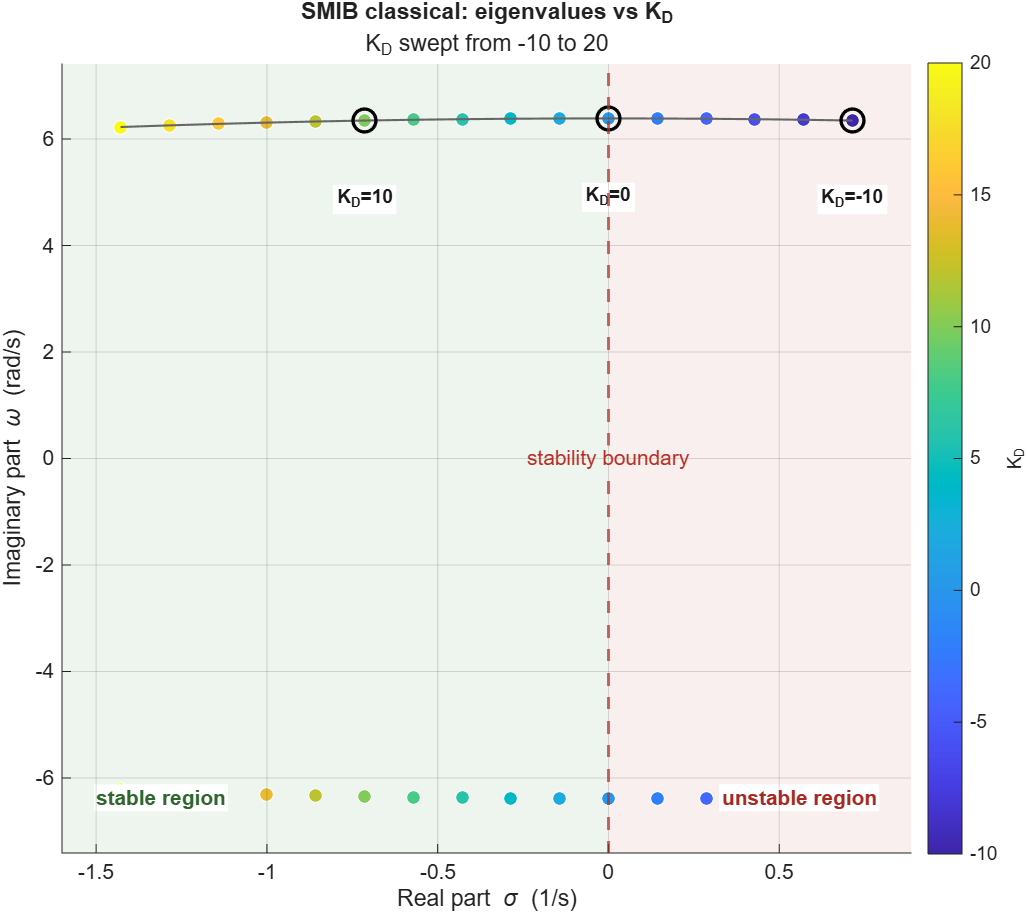
\includegraphics[width=0.85\textwidth]{figures/01_root_locus.png}
\caption{แผนภาพค่าลักษณะเฉพาะหรือ root locus ของแบบจำลอง SMIB แบบ classical
เมื่อกวาดสัมประสิทธิ์การหน่วง $K_D$ จาก $-10$ ถึง $+20$
ครึ่งระนาบซ้ายที่แรเงาคือบริเวณเสถียร และครึ่งระนาบขวาคือบริเวณไม่เสถียร
แกนจินตภาพเส้นประคือขอบเสถียรภาพ ($\sigma=0$)
เมื่อเพิ่มการหน่วงบวก $K_D$ ค่าลักษณะเฉพาะของโหมดสวิงจะเลื่อนไปทางซ้ายเข้าสู่บริเวณเสถียร
ขณะที่การหน่วงลบเลื่อนไปทางขวาเข้าสู่บริเวณไม่เสถียร
จุดที่ทำเครื่องหมายสอดคล้องกับ $K_D=-10$, $0$ และ $+10$}
\label{fig:rootlocus}
\end{figure}

\begin{figure}[H]
\centering
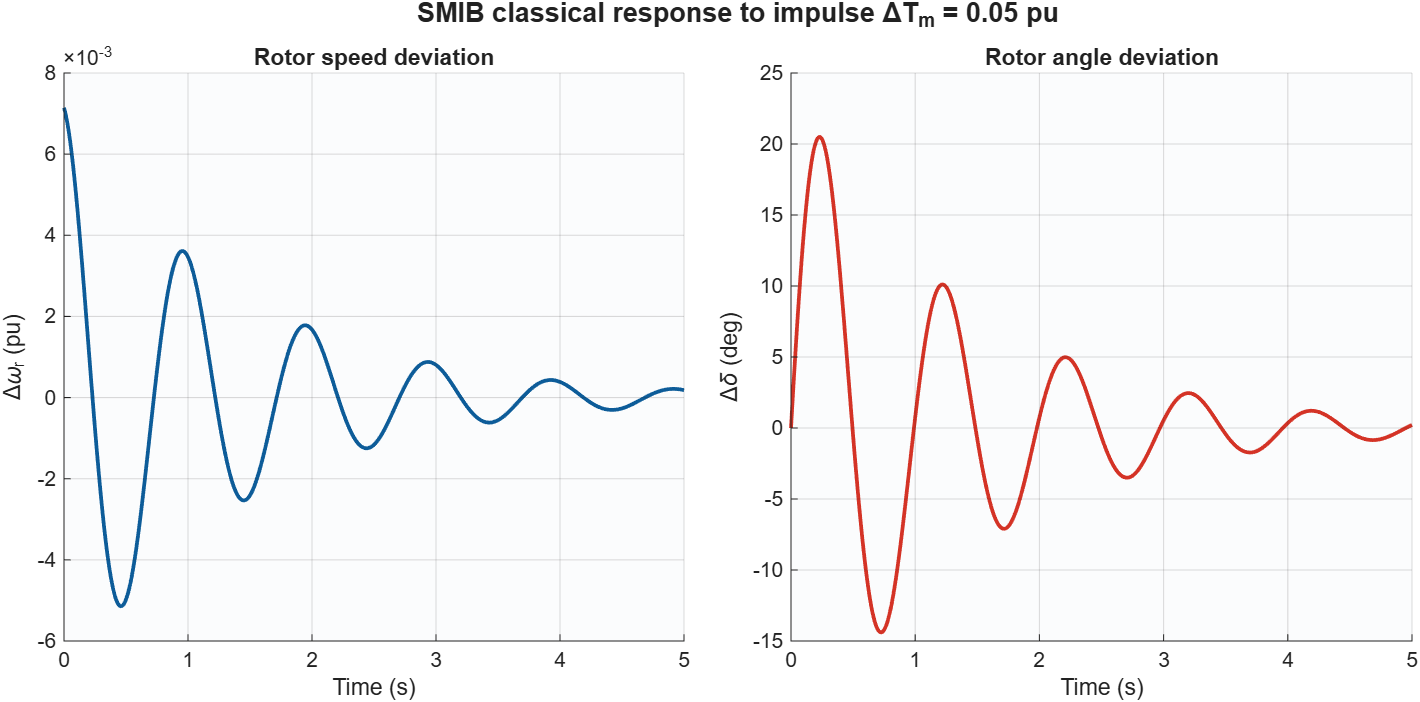
\includegraphics[width=0.9\textwidth]{figures/02_step_response.png}
\caption{ผลตอบสนองโดเมนเวลาของแบบจำลอง classical ($K_D=10$)
ต่อการรบกวนแรงบิดขนาดเล็ก ซ้าย: การเบี่ยงเบนความเร็วโรเตอร์ $\dwr$
ซึ่งลดลงสู่ศูนย์เมื่อโรเตอร์กลับสู่ความเร็วซิงโครนัส
ขวา: การเบี่ยงเบนมุมโรเตอร์ $\ddel$
ซึ่งมีการสั่นลดลงที่ประมาณ $1$~Hz ($\zeta=0.112$)
แสดงว่าเครื่องกำเนิดยังคงซิงโครไนซ์กับบัสอนันต์}
\label{fig:step}
\end{figure}

\begin{figure}[H]
\centering
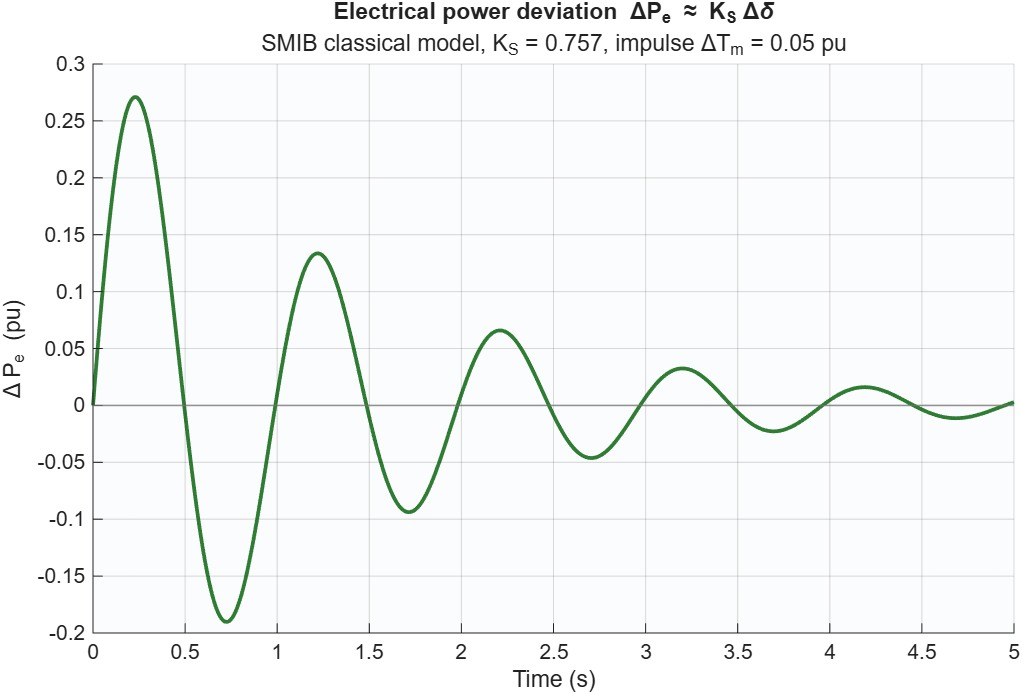
\includegraphics[width=0.7\textwidth]{figures/05_power_response.png}
\caption{ผลตอบสนองกำลังไฟฟ้าของแบบจำลอง classical ($K_D=10$)
ต่อการรบกวนเดียวกัน โดยคำนวณจาก $\Delta P_e \approx K_S\,\ddel$
การสั่นของกำลังที่ลดลงยืนยันว่าเครื่องกลับสู่การส่งกำลังสภาวะคงตัวกับบัสอนันต์
ซึ่งเป็นลายเซ็นในโดเมนเวลาของระบบเสถียรสัญญาณเล็ก}
\label{fig:power}
\end{figure}

\begin{figure}[H]
\centering
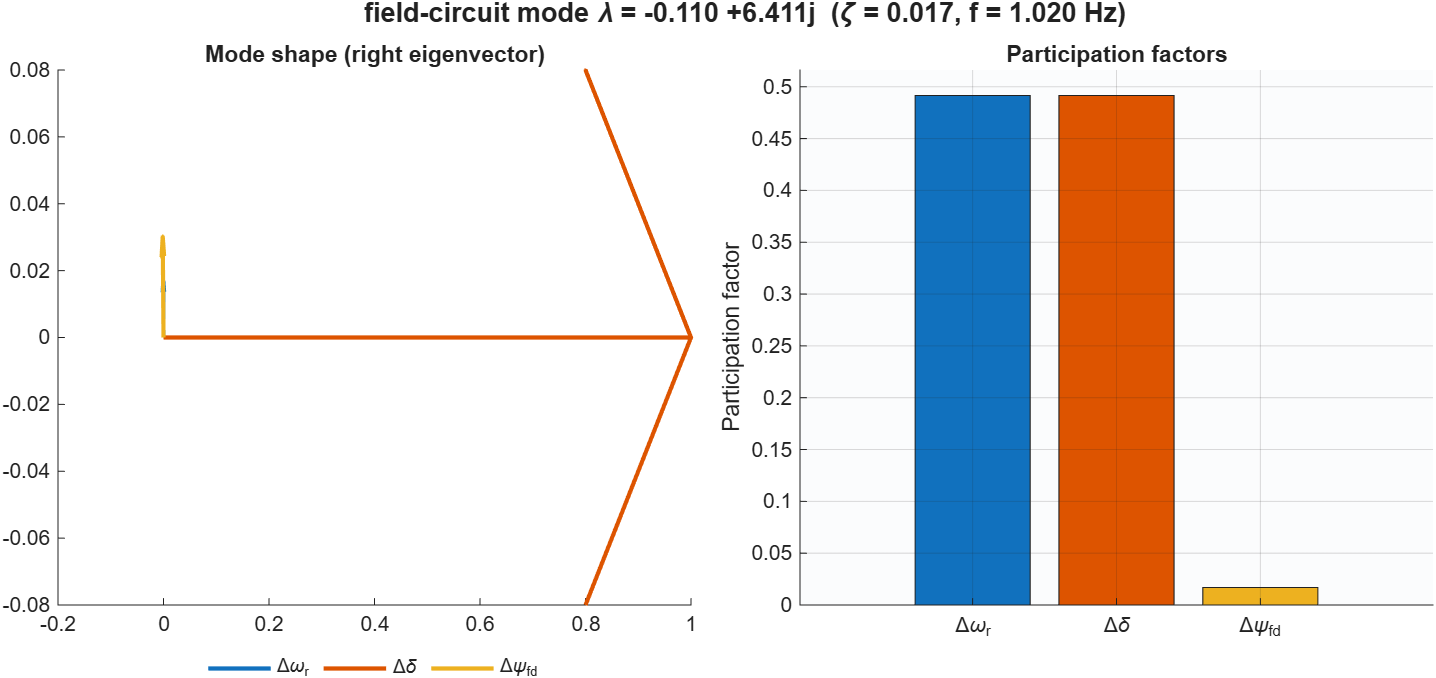
\includegraphics[width=0.9\textwidth]{figures/03_mode_shape.png}
\caption{รูปร่างโหมด (ซ้าย) และ participation factor (ขวา) ของโหมดสวิงแบบ field-circuit
สถานะโรเตอร์ $\dwr$ และ $\ddel$ ครอบงำโหมดเชิงกลไฟฟ้า
ส่วนฟลักซ์สนาม $\dpsifd$ มีส่วนร่วมน้อยมาก
จึงยืนยันการระบุโหมดตามตาราง~\ref{tab:partic}}
\label{fig:modeshape}
\end{figure}

\begin{figure}[H]
\centering
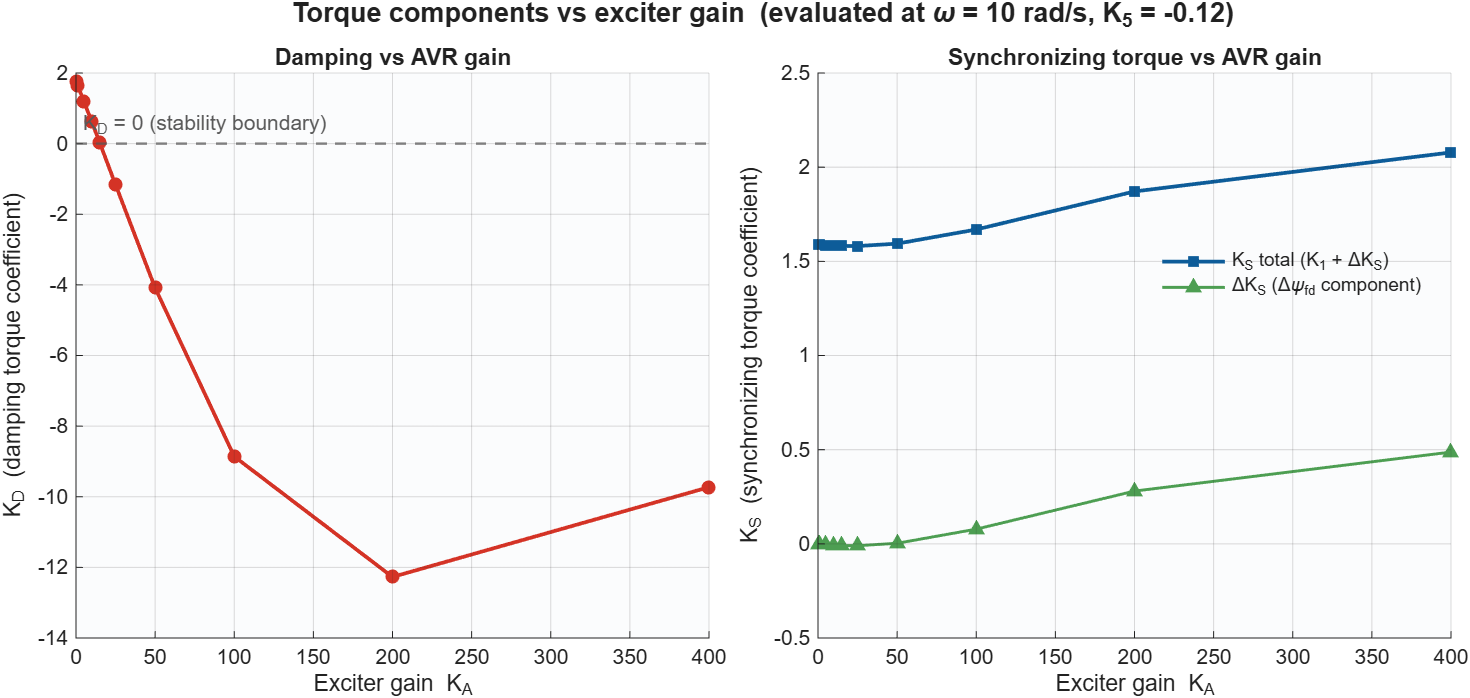
\includegraphics[width=0.9\textwidth]{figures/04_torque_vs_ka.png}
\caption{สัมประสิทธิ์แรงบิดหน่วง (ซ้าย) และแรงบิดซิงโครไนซ์ (ขวา) เทียบกับอัตราขยาย AVR
$K_A$ เมื่อ $K_5<0$ การเพิ่มอัตราขยายเพิ่มแรงบิดซิงโครไนซ์ $K_S$
แต่ผลักแรงบิดหน่วง $K_D$ ให้เป็นลบ ซึ่งทำซ้ำผลของ Kundur ตาราง 12.1
การหน่วงลบคือกลไกที่ทำให้ AVR อัตราขยายสูงทำลายเสถียรภาพของโหมดสวิง}
\label{fig:torque}
\end{figure}

\begin{figure}[H]
\centering
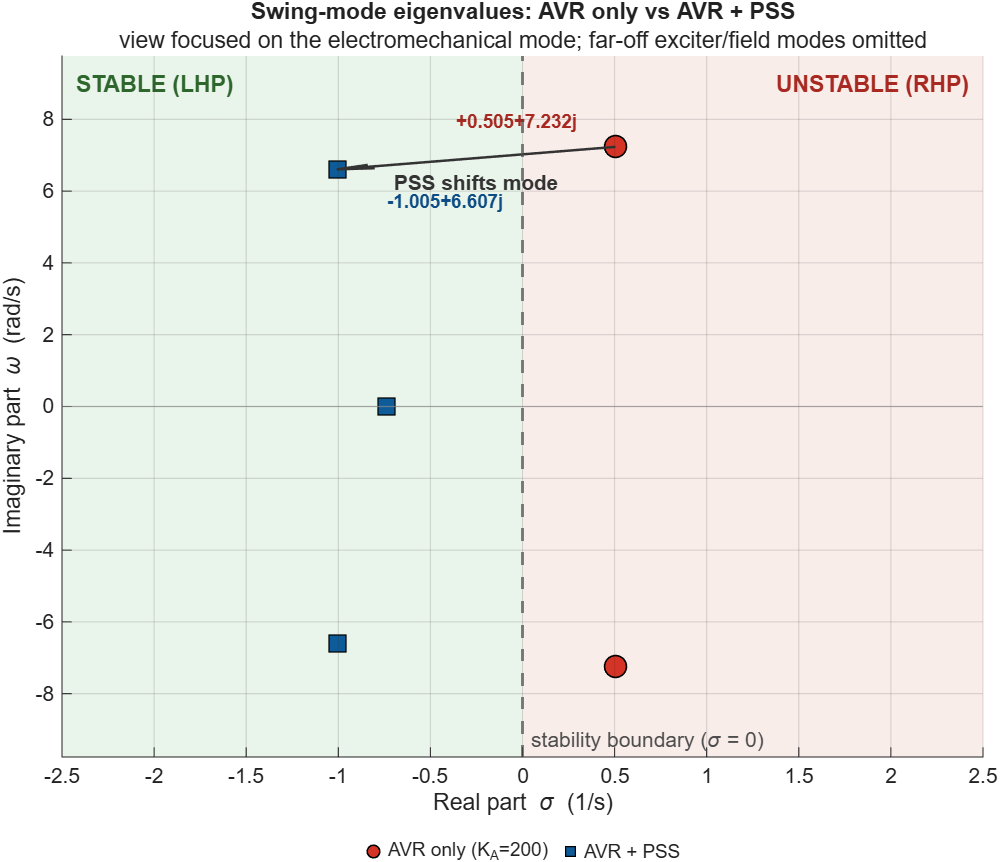
\includegraphics[width=0.8\textwidth]{figures/06_eig_comparison.png}
\caption{ค่าลักษณะเฉพาะของโหมดสวิงเมื่อมีเฉพาะ AVR (ครึ่งระนาบขวา,
$+0.504\pm j7.23$, ไม่เสถียร) และเมื่อมี AVR\,+\,PSS (ครึ่งระนาบซ้าย,
$-1.005\pm j6.607$, เสถียร) ที่ $K_A=200$
PSS ย้ายโหมดเชิงกลไฟฟ้าข้ามขอบเสถียรภาพเข้าสู่บริเวณเสถียร
ภาพนี้โฟกัสที่โหมดสวิง ส่วนโหมดตัวกระตุ้นและสนามที่อยู่ไกลออกไปอยู่นอกกรอบภาพ}
\label{fig:eigcmp}
\end{figure}

\noindent
ตาราง~\ref{tab:figinterp} สรุปวิธีอ่านรูปแต่ละรูปในเชิงเสถียรภาพ

\begin{table}[H]
\centering
\caption{การตีความรูปประกอบในเชิงเสถียรภาพสัญญาณเล็ก}
\label{tab:figinterp}
\renewcommand{\arraystretch}{1.3}
\newcolumntype{Y}{>{\raggedright\arraybackslash}X}
\begin{tabularx}{\textwidth}{@{}>{\raggedright\arraybackslash\hyphenpenalty=10000\exhyphenpenalty=10000}p{4.3cm}Y Y@{}}
\toprule
\textbf{รูป} & \textbf{สิ่งที่แสดง} & \textbf{การตีความเสถียรภาพ} \\
\midrule
แผนภาพค่าลักษณะเฉพาะ / root locus (รูป~\ref{fig:rootlocus})
 & การเคลื่อนที่ของค่าลักษณะเฉพาะเมื่อ $K_D$ เปลี่ยน
 & ครึ่งระนาบซ้าย $\Rightarrow$ เสถียร; ครึ่งระนาบขวา $\Rightarrow$ ไม่เสถียร \\
ผลตอบสนองมุมโรเตอร์ (รูป~\ref{fig:step}, ขวา)
 & การสั่นของ $\ddel$
 & การสั่นที่ลดลง $\Rightarrow$ ยังคงซิงโครไนซ์ \\
ผลตอบสนองความเร็วโรเตอร์ (รูป~\ref{fig:step}, ซ้าย)
 & การสั่นของ $\dwr$
 & กลับสู่ศูนย์ $\Rightarrow$ ความเร็วกลับสู่ซิงโครนัส \\
ผลตอบสนองกำลังไฟฟ้า (รูป~\ref{fig:power})
 & การสั่นของ $\Delta P_e$
 & การสั่นกำลังที่ลดลง $\Rightarrow$ การส่งกำลังเสถียร \\
ผลของอัตราขยาย AVR (รูป~\ref{fig:torque})
 & $K_S$ และ $K_D$ เทียบกับ $K_A$
 & อัตราขยายสูงเพิ่ม $K_S$ แต่อาจลด $K_D$ \\
ค่าลักษณะเฉพาะ AVR เทียบ PSS (รูป~\ref{fig:eigcmp})
 & โหมดสวิงก่อนและหลังเพิ่ม PSS
 & PSS ย้ายโหมดไปยังครึ่งระนาบซ้ายที่เสถียร \\
\bottomrule
\end{tabularx}
\end{table}

\section{อภิปรายผล}
\label{sec:discussion}

แบบจำลองทั้งสี่เล่าเรื่องเดียวกันอย่างเป็นลำดับเกี่ยวกับเสถียรภาพมุมโรเตอร์สัญญาณเล็ก

\begin{itemize}
    \item \textbf{แบบจำลอง classical} แบบจำลองนี้กำหนดความถี่สวิงเชิงกลไฟฟ้าพื้นฐานใกล้ $1$~Hz
          ซึ่งถูกกำหนดโดยสัมประสิทธิ์ซิงโครไนซ์ $K_S$ และความเฉื่อย $H$
          (สมการ~\ref{eq:wn}) เมื่อไม่มีการหน่วง ($K_D=0$) โหมดอยู่บนแกนจินตภาพพอดี
    \item \textbf{บทบาทของ $K_D$} $K_D$ บวกย้ายค่าลักษณะเฉพาะของโหมดสวิงเข้าสู่ครึ่งระนาบซ้าย
          (ถูกหน่วงและเสถียร) ส่วน $K_D$ ลบย้ายเข้าสู่ครึ่งระนาบขวา
          (การสั่นขยายตัวและไม่เสถียร) root locus ในรูป~\ref{fig:rootlocus}
          แสดงพฤติกรรมนี้โดยตรง
    \item \textbf{พลวัตวงจรสนาม} การเพิ่มฟลักซ์สนามสร้างการหน่วง \emph{บวก} เล็กน้อยให้โหมดสวิง
          ($\zeta\approx0.017$) และสร้างโหมดสนามไม่สั่นที่มีการหน่วงดี
          โหมดเชิงกลไฟฟ้ายังคงระบุได้ชัดจาก participation factor
    \item \textbf{AVR อัตราขยายสูง} AVR แบบไทริสเตอร์ปรับปรุงการควบคุมแรงดันและแรงบิดซิงโครไนซ์อย่างมาก
          แต่เพราะ $K_5<0$ ที่โหลดนี้ จึงฉีดแรงบิดหน่วง \emph{ลบ}
          ที่ $K_A=200$ สัมประสิทธิ์การหน่วงถึง $-12.3$
          และโหมดสวิงข้ามเข้าสู่ครึ่งระนาบขวา ($+0.504\pm j7.23$):
          ตัวควบคุมทำให้โหมดโรเตอร์ไม่เสถียร
    \item \textbf{Power system stabilizer} PSS เพิ่มสัญญาณเสริมจากการเบี่ยงเบนความเร็ว
          ผ่าน washout และเครือข่าย lead-lag ที่ชดเชยเฟส เข้าสู่จุดรวมของตัวกระตุ้น
          วิธีนี้คืนการหน่วงบวกและย้ายโหมดสวิงกลับสู่ครึ่งระนาบซ้าย
          ($-1.005\pm j6.607$, $\zeta=0.15$) ดังที่รูป~\ref{fig:eigcmp} แสดง
\end{itemize}

ลำดับนี้ชี้ให้เห็นข้อแลกเปลี่ยนพื้นฐานในการควบคุมการกระตุ้น:
อัตราขยายสูงชุดเดียวกันที่เสริมแรงบิดซิงโครไนซ์และการควบคุมแรงดัน
อาจกัดกร่อนการหน่วงได้ และตัวรักษาเสถียรภาพเฉพาะทางคือวิธีแก้มาตรฐาน

\section{สรุป}

เสถียรภาพสัญญาณเล็กของระบบเครื่องกำเนิดเดี่ยวต่อบัสอนันต์ถูกวิเคราะห์ใน 4 ระดับรายละเอียด
ด้วยแบบจำลอง state-space ลิเนียไรซ์และการวิเคราะห์ค่าลักษณะเฉพาะ
พร้อมใช้ผลตอบสนองโดเมนเวลายืนยันคำทำนายจากค่าลักษณะเฉพาะตลอดทั้งรายงาน
เมทริกซ์สถานะของแต่ละแบบจำลองประกอบจากพารามิเตอร์เครื่องจักรและเครือข่าย
โดยค่าคงที่ Heffron--Phillips $K$ ถูกอนุมานจากข้อมูล $d$--$q$ และการอิ่มตัวตั้งแต่หลักการพื้นฐาน
จากนั้นใช้โครงสร้างค่าลักษณะเฉพาะเพื่อตัดสินเสถียรภาพและวัดการหน่วงกับความถี่ของโหมดเชิงกลไฟฟ้า

การวิเคราะห์ยืนยันข้อสรุปสำคัญของเสถียรภาพมุมโรเตอร์:
state-space และค่าลักษณะเฉพาะประเมินเสถียรภาพสัญญาณเล็กของ SMIB ได้โดยตรงจากส่วนจริงของค่าลักษณะเฉพาะ
ผลตอบสนองเวลาในมุมโรเตอร์ ความเร็ว และกำลังไฟฟ้ายืนยันผลเหล่านั้น
AVR อัตราขยายสูงปรับปรุงการควบคุมแรงดันและแรงบิดซิงโครไนซ์
แต่เมื่อ $K_5<0$ อาจลดการหน่วงและทำให้โหมดสวิงไม่เสถียร
และ PSS ที่ปรับแต่งเหมาะสมจะคืนการหน่วงบวกและย้ายโหมดสวิงที่ไม่เสถียรกลับสู่ครึ่งระนาบซ้ายที่เสถียร
ผลเชิงตัวเลขทุกค่า ได้แก่ ความถี่สวิง classical $1.02$~Hz,
ค่าลักษณะเฉพาะของวงจรสนาม, แนวโน้มแรงบิดหน่วงของ AVR ในตาราง~12.1,
และการทำให้เสถียรด้วย PSS จาก $+0.504\pm j7.23$ เป็น $-1.005\pm j6.607$
สอดคล้องกับตัวอย่างที่เกี่ยวข้องใน Kundur บทที่ 12

\begin{thebibliography}{9}
\bibitem{kundur} P. Kundur, \textit{Power System Stability and Control},
McGraw-Hill, 1994. Chapter 12 (Examples 12.2, 12.3, 12.6; Section 12.4,
Table 12.1).
\bibitem{anderson} P. M. Anderson and A. A. Fouad, \textit{Power System Control
and Stability}, 2nd ed., IEEE Press / Wiley, 2003.
\bibitem{sauer} P. W. Sauer and M. A. Pai, \textit{Power System Dynamics and
Stability}, Prentice Hall, 1998.
\end{thebibliography}

\end{document}
